\documentclass[english,onecolumn]{IEEEtran}
\usepackage[T1]{fontenc}
\usepackage[latin9]{luainputenc}
\usepackage[letterpaper]{geometry}
\geometry{verbose}
\usepackage{amsfonts}
\usepackage{babel}

\usepackage{extarrows}
\usepackage[colorlinks]{hyperref}
\usepackage{listings}
\usepackage{xcolor}
\usepackage[ruled,linesnumbered]{algorithm2e}

\usepackage{amsmath,graphicx}
\usepackage{subfigure} 
\usepackage{cite}
\usepackage{amsthm,amssymb,amsfonts}
\usepackage{textcomp}
\usepackage{bm}
\usepackage{booktabs}
\usepackage{listings}
\definecolor{salmon}{rgb}{1, 0.5020, 0.4471}
\usepackage{xparse}

\NewDocumentCommand{\codeword}{v}{%
\texttt{\textcolor{blue}{#1}}%
}

\lstdefinestyle{mystyle}{
    numberstyle=\color{green},
    numbers=left,                    
    numbersep=5pt,                  
    showspaces=false,                
    showstringspaces=false,
    showtabs=false,                  
    tabsize=2
}

\lstset{style=mystyle}

\providecommand{\U}[1]{\protect\rule{.1in}{.1in}}
\topmargin            -18.0mm
\textheight           226.0mm
\oddsidemargin      -4.0mm
\textwidth            166.0mm
\def\baselinestretch{1.5}


\newcommand{\Rbb}{\mathbb{R}}
\newcommand{\Pb}{\mathbf{P}}
\newcommand{\Ib}{\mathbf{I}}
\newcommand{\vb}{\mathbf{v}}
\newcommand{\Ucal}{\mathcal{U}}
\newcommand{\Wcal}{\mathcal{W}}
\newcommand{\Vcal}{\mathcal{V}}
\newcommand{\Rcal}{\mathcal{R}}
\newcommand{\Ncal}{\mathcal{N}} 


\def\Q{\mathbf{Q}}
\def\A{\mathbf{A}}
\def\R{\mathbf{R}}
\def\I{\mathbf{I}}


\begin{document}

\begin{center}
	\textbf{\LARGE{SI231 - Matrix Computations, Fall 2020-21}}\\
	{\Large Homework Set \#3}\\
	\texttt{Prof. Yue Qiu and Prof. Ziping Zhao}\\
	\texttt{\textbf{Name:}}   	\texttt{ Tian Yun }  		\hspace{1bp}
	\texttt{\textbf{Major:}}  	\texttt{ Master in CS } 	\\
	\texttt{\textbf{Student No.:}} 	\texttt{ 2019232102}     \hspace{1bp}
	\texttt{\textbf{E-mail:}} 	\texttt{ tianyun@shanghaitech.edu.cn}
\par\end{center}



\noindent
\rule{\linewidth}{0.4pt}
{\bf {\large Acknowledgements:}}
\begin{enumerate}
    \item Deadline: \textbf{2020-11-01 23:59:00}
    \item Submit your homework at \textbf{Gradescope}. Entry Code: \textbf{MY3XBJ}. 
    Homework \#3 contains two parts, the theoretical part the and the programming part.
    \item About the the theoretical part:
    \begin{enumerate}
            \item[(a)] Submit your homework in \textbf{Homework 3} in gradescope. Make sure that you have correctly select pages for each problem. If not, you probably will get 0 point.
            \item[(b)] Your homework should be uploaded in the \textbf{PDF} format, and the naming format of the file is not specified.
            \item[(c)] You need to use \LaTeX $\,$ in principle.
            \item[(d)] Use the given template and give your solution in English. Solution in Chinese is not allowed. 
        \end{enumerate}
  \item About the programming part:
  \begin{enumerate}
      \item[(a)] Submit your codes in \textbf{Homework 3 Programming part} in gradescope.
      \item[(b)] Detailed requirements see in Problem 2 and Probelm 3.
  \end{enumerate}
  \item \textbf{No late submission is allowed.}
\end{enumerate}
\rule{\linewidth}{0.4pt}
\newpage 

\section{Understanding projection}
\noindent\textbf{Problem 1}. \textcolor{blue}{(5 points $\times$ 3)}

Suppose that $\Pb\in \Rbb^{n\times n}$ is a projector onto a subspace $\mathcal{U}$ along its orthogonal complement $\mathcal{U}^{\perp}$, then it is called the \textbf{orthogonal projector} onto $\Ucal$.
\begin{enumerate}
    \item Prove that an orthogonal projector must be singular if it is not an identity matrix.
	\item What is the orthogonal projector onto $\mathcal{U}^{\perp}$ along the subspace $\mathcal{U}$?
    \item Let $\Ucal$ and $\Wcal$ be two subspaces of a vector space $\mathcal{V}$, and denote $\Pb_{\Ucal}$ and $\Pb_{\Wcal}$ as the corresponding orthogonal projectors, respectively. Prove that $\Pb_{\Ucal} \Pb_{\Wcal} = 0$ if and only if $\Ucal \perp \Wcal$.
\end{enumerate}

\noindent
\textbf{Solution.}
\begin{enumerate}
	\item $\textbf{proof}$:
	A projection on a vector space $V$ is a linear operator $P: V \mapsto V$ such that $P^{2}=P$.$\quad P \in R^{n \times m}$
	
	$\therefore P(I-P) = 0$, and $rank(P(I-P))) = 0$. 
	
	$\therefore rank(P) + rank(I-p) - n \leq 0$
	
	$\therefore rank(P) + rank(I-p)  \leq n$
	
	First case : $rank(p) = n$, $\quad \therefore rank(I-p) = 0, \therefore I=p$
	
	Second case: $rank(p) \leq n$, $\quad \therefore$ p must be singular.
	
	\item $\textbf{I} -\Pb$.
	
	$\Pb\in \Rbb^{n\times n}$ is a projector onto a subspace $\mathcal{U}$ along its orthogonal complement $\mathcal{U}^{\perp}$
	
	so for all $x \in \mathcal{U}$,  $\Pb x = x$, for all $x \in \mathcal{U}^{\perp}$, $\Pb x = 0$
	
	Now we want to find the orthogonal projector $\Pb^*$ onto $\mathcal{U}^{\perp}$ along the subspace $\mathcal{U}$
	
	it means for all $y \in \mathcal{U^{\perp}}$,  $\Pb^* y = y$, for all $y \in \mathcal{U}$, $\Pb^* y = 0$
	
	$\Pb^* = \textbf{I} -\Pb$.
	
	because for all $x \in \mathcal{U}^{\perp}$ , $(\textbf{I} -\Pb)x = x$ and for all $x \in \mathcal{U}$ , $(\textbf{I} -\Pb)x = 0$, satisfied with the  analysis above.
	
	\item $\textbf{proof}$: 
	
	
	On the one hand, $\forall x_u \in \mathcal{U} , \exists x \in \mathcal{V}$ s.t. $ x_{u} = \Pb_{\Ucal} x \quad \forall x_w \in \mathcal{W} ,\exists y \in \mathcal{V}$ s.t. $ y_{w} =\Pb_{\Wcal}  y$  . 
	
	if $\Pb_{\Ucal} \Pb_{\Wcal}  = 0$ , and $\Pb_{\Ucal}  x_{u} = 0$ , $\Pb_{\Wcal}  y_{w} = 0$ so $x_{u}^T \Pb_{\Ucal}^T \Pb_{\Wcal} x_{w}= 0$
		
	So for any $z_u \in \Ucal$  and because for any $z_w \in \Wcal \quad z_u^T  \perp z_w$
	
	$\therefore \Ucal \perp \Wcal$
	
	On the other hand, if $\Ucal \perp \Wcal$   So for any $z_u \in \Ucal$  and for any $z_w \in \Wcal \quad z_u^T z_w = 0$
	
	so for any $z_{u} \in \mathcal{U}$, we can find a vector $x \in V$ s.t. $\Pb_{\Ucal} x = z_u$ 
	
	and for any $z_{v} \in \mathcal{V}$ we can find a vector $y \in V$ s.t. $\Pb_{\Wcal} y = z_w$ 
	
	$\because z_u^T z_w = 0$, therefore $(\Pb_{\Ucal} x)^T \Pb_{\Wcal} y = 0$
	
	So $x^T \Pb_{\Ucal}^T \Pb_{\Wcal} y = 0$ 
	
	$\therefore \Pb_{\Ucal}^T \Pb_{\Wcal} = 0$ 


%	because $\Ucal$ and $\Wcal$  are the subspace of $\Vcal$,so $z = x_{u} + y_{w} \in \Vcal$ 
\end{enumerate}

\newpage
\section{Least Square (LS) programming.}
\noindent\textbf{Problem 2}. \textcolor{blue}{(10 points + 10 points + 5 points)}

Write programs to solve the least square problem with specified methods, any programming language is suitable.
$$
\mathbf{x} = \mathop{\arg\min}_{\mathbf{x} \in \Rbb^n} f(\mathbf{x}), \quad f(\mathbf{x}) = ||\mathbf{y}-\mathbf{A}\mathbf{x}||_2^2
$$
where $\mathbf{A} \in \Rbb^{m \times n}$ is a matrix representing the predefined data set with $m$ data samples of $n$ dimensions ($m$=1000, $n$=210), and $\mathbf{y} \in \Rbb^m$ represents the labels. The data samples are provided in the "data.txt" file, and the labels are provided in the "label.txt" file, you are supposed to load the data before solving the problem.

\begin{enumerate}
    \item Solve the LS with gradient decent method.\\
    The gradient descent method for solving problem updates $ {\bf x}$ as
    $$
        {\bf x} = {\bf x} - \gamma \cdot \nabla_{{\bf x}} f(\mathbf{x}),
    $$
    where $\gamma$ is the step size of the gradient decent methods. We suggest that you can set $\gamma=1e-5$.
    \item Solve the LS by the method of normal equation with Cholesky decomposition and forward/backward substitution.
    \item Compare two methods above. 
    \begin{enumerate}
        \item[(a)] Basing on the true running results from the program, count the number of "flops"*;
        \item[(b)] Compare gradient norm and loss $f(\mathbf{x})$ for results $\mathbf{x}=\mathbf{x_{LS}}$ of above two algorithms.
    \end{enumerate}
\end{enumerate}
    \textbf{Notation*:} "flop": one flop means one floating point operation, i.e., one addition, subtraction, multiplication, or division of two floating-point numbers, in this problem each floating points operation $+,-,\times, \div, \sqrt{\cdot}$ counts as one "flop". \\
    \textbf{Hint for gradient decent programming:} 
    \begin{enumerate}
        \item \textbf{Step size selection}: to ensure the convergence of the method, $\gamma$ is supposed to be selected properly (large step size may accelerate the convergence rate but also may lead to instability, A sufficiently small compensation always ensures that the algorithm converges). 
        \item \textbf{Terminal condition}: the gradient decent is an iteration algorithm that need a terminal condition. In this problem, the algorithm can stop when the gradient of the loss function $f(\mathbf{x})$ at current $\mathbf{x}$ is small enough.
    \end{enumerate}
    \noindent\textbf{Remarks: }
   \begin{itemize}
    \item The solution of the two methods should be printed in files named "sol1.txt" and "sol2.txt" and submitted in gradescope.  The format should be same as the input file (210 rows plain text, each rows is a dimension of the final solution).
    \item Make sure that your codes are executable and are consistent with your solutions.
   \end{itemize}
\noindent
\textbf{Solution.}

1).You can check in my uploaded  file.

2).You can check in my uploaded  file.

3). (a)

n = 210 , m = 1000

(1).Gradient descent method:

The stop condition used here is that the change value of cost is less than 1e-6, and a total of k = 85 iterations are performed.

Each iteration needs to be calculated:

1. $X*theta$

2. $X' * (predictions - y)$

3. $theta = theta - alpha * updates$

Assuming that C iterations are required to complete, the time complexity of each iteration is $f l o p_{i}=n^{2} m+n^{2}+m n+3 n$ 

(2). Normal Equations:

1. $L = chol(X' * X);$

2. $temp = forwardsub(L',X'*y);$

3. $theta = backwardsub(L,temp);$

chol: A total of $O\left(n^{2}\right)$ elements are calculated, and the calculation of each element contains the multiplication of $O(n)$, so it is $O\left(n^{ 3}\right)$

 For forward substitution and backward substitution algorithms, since L or L'is a triangular matrix, the first one can be calculated in the order of $y_{1}, y_{2}, \cdots$, the required calculation The complexity is $O\left(n^{2}\right),$ Similarly, the third one can also be calculated like this.

So the total computational complexity is $O\left(n^{3}+n^{2}\right)=O\left(n^{3}\right)$ flops .The advantage of this algorithm is that when it is necessary to solve different x with relatively different b for the same A, the new part can be completed with $O\left(n^{2}\right)$ complexity.

(b)
\begin{figure}[!htb]
	\centering
	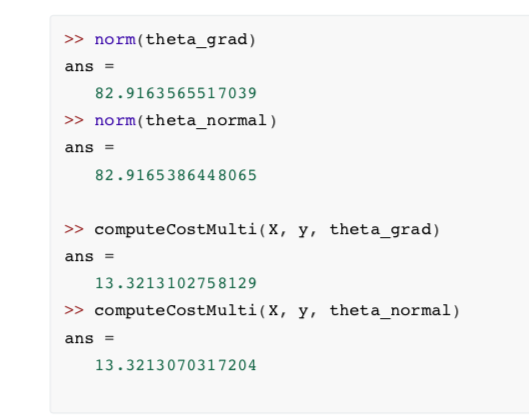
\includegraphics[scale=0.35]{norm.png}
\end{figure}

theta\_grad is the result of gradient descent and theta\_norm is the result of norm equation.

norm() fuction will calculate the L2 norm of the vector,and computeCostMulti() function will calculate the loss for $f(x)$

\newpage
\section{Understanding the QR Factorization}
\noindent\textbf{Problem 3 [Understanding the Gram-Schmidt algorithm.]}. \textcolor{blue}{(5 points + 7 points + 6 points + 7 points)}
\begin{enumerate}
	\item 
	Consider the subspace $\mathcal{S}$ spaned by $\{ {\bf a}_1,\ldots, {\bf a}_4\}$, where
	\[
	{\bf a}_1 = \begin{bmatrix} 1 \\ 2 \\ 3 \\ 4\end{bmatrix}\,,\quad 
	{\bf a}_2 =  \begin{bmatrix}2 \\ 3 \\ 4 \\ 5 \end{bmatrix}\,,\quad 
	{\bf a}_3 =  \begin{bmatrix}3 \\ 4 \\5 \\ 6 \end{bmatrix}\,,\quad
	{\bf a}_4 =  \begin{bmatrix}3 \\ 5 \\7 \\ 11 \end{bmatrix}\,.
	\] 
	Use the \textbf{classical} Gram-Schimidt algorithm (See Algorithm \ref{alg:classical_gs}), find a set of orthonormal basis $\{{\bf q}_i\}$ for $\mathcal{S}$ by hand (derivation is expected). \textcolor{black}{
	Do not use decimals in your answers, fraction and $n$-th roots of numbers are accepted.}
	Verify the orthonormality of the found basis.
	\begin{algorithm}[htbp]
 \label{alg:classical_gs}
\SetKwInOut{Input}{Input}\SetKwInOut{Output}{Output}
\caption{Classical Gram-Schmidt algorithm}
\SetAlgoLined
\Input{A collection of linearly independent vectors ${\bf a}_1,\ldots, {\bf a}_n$.}
\textbf{Initilization:} $\widetilde{{\bf q}}_1 = {\bf a}_1, {\bf q}_1 = \widetilde{{\bf q}}_1/\|\widetilde{{\bf q}}_1\|_2$\\
 \For{$i= 2,\ldots, n$}{
  $\widetilde{{\bf q}}_i = {\bf a}_i - \sum_{j=1}^{i-1} ({\bf q}_j^T{\bf a}_i){\bf q}_j$\\
  ${\bf q}_i = \widetilde{{\bf q}}_i/\|\widetilde{{\bf q}}_i\|_2$ 
 }
 \Output{${\bf q}_1,\ldots, {\bf q}_n$}
\end{algorithm}
	\item 
	Orthogonal projection of vector ${\bf a}$ onto a nonzero vector ${\bf b}$ is defined as
	\[
	\text{proj}_\mathbf{b}(\bf a)=\frac{\langle{\bf a},{\bf b}\rangle}{\langle{\bf b},{\bf b}\rangle}{\bf b},
	\]
	where $\langle,\rangle$ denotes the inner product of vectors.
	And for subspace $\mathcal{M}$ with 
	orthonormal basis $\{ {\bf u}_1,\ldots, {\bf u}_k \}$, the orthogonal projector onto subspace $\mathcal{M}$ is given by 
	\[
	{\bf P} = {\bf UU}^T\,,\quad {\bf U} = [{\bf u}_1|\cdots|{\bf u}_k]\,.
	\]
	In the context of \textbf{projection of vector} and \textbf{projection onto subspace} respectively, can you give another two understandings of the classical Gram-Schmidt algorithm?
    %Try to understand Gram-Schmidt algorithm in the context of \textbf{projection onto subspace} and give a new expression of ${\bf q}_k$ based on your understanding.
	%It can b \|\,,\\_2e written as projection of subspace $\bf Pa$ and $\bf P$ is an orthogonal projector, where $\bf P$ is a projection matrix.
	\item Consider the subspace $\mathcal{S}$ spaned by $\{{\bf a}_1, {\bf a}_2, {\bf a}_3\}$,
	\[
	{\bf a}_1 = \begin{bmatrix} 1 \\ \epsilon \\ \epsilon \\ \end{bmatrix}\,,\quad 
	{\bf a}_2 =  \begin{bmatrix}1 \\ \epsilon \\ 0\end{bmatrix}\,,\quad 
	{\bf a}_3 =  \begin{bmatrix}1 \\ 0 \\ \epsilon\end{bmatrix}\,,
	\]
	where $\epsilon$ is a small real number such that $1+k\epsilon^2 =1$ $(k\in\mathbb{N}^+)$. 
	First complete the pseudo algorithm in Algorithm \ref{alg:modified_gs}.
	Then use the \textbf{classical} Gram-Schimidt algorithm and the \textbf{modified} Gram-Schimidt algorithm respectively, find two sets of basis for $\mathcal{S}$ by hand (derivation is expected). Are the two sets of basis the same? If not, which one is the desired orthonormal basis? Report what you have found.
	\begin{algorithm}[htbp]
	\label{alg:modified_gs}
\SetKwInOut{Input}{Input}\SetKwInOut{Output}{Output}
\caption{Modified Gram-Schmidt algorithm}
\SetAlgoLined
\Input{A collection of linearly independent vectors ${\bf a}_1,\ldots, {\bf a}_n$.}
\textbf{Initilization:}\\
\textbf{\textit{Complete your algorithm here...}}\\
 \Output{${\bf q}_1,\ldots, {\bf q}_n$}
\end{algorithm}
	\item \textbf{Programming part:}
	In this part, you are required to code both the \textbf{ classical Gram-Schmidt} and \textbf{the modified Gram-Schmidt} algorithms.
	For $\epsilon=1\text{e}-4$ and $\epsilon=1\text{e}-9$ in sub-problem 2), give the outputs of two algorithms and calculate $\|{\bf Q}^T {\bf Q} - {\bf I}\|_{\text{F}}$, where ${\bf Q} = [{\bf q}_1,{\bf q}_2,{\bf q}_3]$.
\end{enumerate}
\noindent\textbf{Remarks: }
\begin{itemize}
    \item Coding languages are not restricted, but do not use built-in function such as \codeword{qr}.
    \item When handing in your homework in gradescope, package all your codes into {\sf your\_student\_id+hw3\_code.zip} and upload. In the package, you also need to include a file named {\sf README.txt/md} to clearly identify the function of each file.
     \item Make sure that your codes can run and are consistent with your solutions.
\end{itemize}

\noindent
\textbf{Solution.}
\begin{enumerate}
	\item 
	1) According to Algorithm
	
	$\tilde{\mathbf{q}}_{1}=\mathbf{a_{1}}=\left[\begin{array}{llll}1 & 2 & 3 & 4\end{array}\right]^{T}$.

$\mathbf{q}_{1}=\tilde{\mathbf{q}}_{1} /\left\|\tilde{\mathbf{q}}_{1}\right\|_{2}=\frac{1}{\sqrt{30}}\left[\begin{array}{llll}1 & 2 & 3 & 4\end{array}\right]^{T}$

$\tilde{\mathbf{q}}_{2}=\mathbf{a}_{2}-\left(\mathbf{q}_{1}^{T} \mathbf{a}_{2}\right) \mathbf{q}_{1}=\left[\begin{array}{llll}2 & 3 & 4 & 5\end{array}\right]^{T}-\frac{1}{3}\left[\begin{array}{llll}4 & 8 & 12 & 16\end{array}\right]^{T}=\frac{1}{3}\left[\begin{array}{llll}2 & 1 & 0 & -1\end{array}\right]^{T}$

$\mathbf{q}_{2}=\tilde{\mathbf{q}}_{2} /\left\|\tilde{\mathbf{q}}_{2}\right\|_{2}=\frac{1}{\sqrt{6}}\left[\begin{array}{llll}2 & 1 & 0 & -1\end{array}\right]^{T}$
	$$\tilde{\mathbf{q_{3}}}=\mathbf{a_{3}}-\left(\mathbf{q_{1}}^{T} \mathbf{a_{3}}\right) \mathbf{q_{1}}-\left(\mathbf{q_{2}}^{T} \mathbf{a_{3}}\right) \mathbf{q_{2}}=0,$$
	So $\left(\mathbf{a}_{1}, \mathbf{a}_{2}, \mathbf{a}_{3}, \mathbf{a}_{4}\right)$ are not linearly independent. We can get the set
	of orthonormal basis from 
	$a_{1}, a_{2}, a_{4}$
	$$
	\tilde{\mathbf{q_{4}}}=\mathbf{a_{4}}-\left(\mathbf{q_{1}}^{T} \mathbf{a_{4}}\right) \mathbf{q_{1}}-\left(\mathbf{q_{2}}^{T} \mathbf{a_{4}}\right) \mathbf{q_{2}}=\frac{1}{5}\left[\begin{array}{ccccc}
		2 & -1 & -4 & 3
	\end{array}\right]^{T}, \quad \mathbf{q_{4}}=\frac{\bar{\mathbf{q}_{4}}}{\left\|\bar{\mathbf{q}}_{4}\right\|}=\frac{\sqrt{30}}{30}\left[\begin{array}{cccc}
		2 & -1 & -4 & 3
	\end{array}\right]^{T}
	$$
	We can get it easily that $\mathbf{q_{1}}^{T} \mathbf{q_{2}}=\mathbf{q_{1}}^{T} \mathbf{q_{4}}=\mathbf{q_{2}}^{T} \mathbf{q_{4}}=0,$ so set of the basis $\mathbf{q_{1}}, \mathbf{q_{2}}, \mathbf{q_{4}}$ is orthonormal basis.
	
$$
\mathbf{Q}=\left[\begin{array}{ccc}
	\frac{1}{\sqrt{30}} & \frac{2}{\sqrt{6}} & \frac{2}{\sqrt{30}} \\
	\frac{2}{\sqrt{30}} & \frac{1}{\sqrt{6}} & -\frac{1}{\sqrt{30}} \\
	\frac{3}{\sqrt{30}} & 0 & -\frac{4}{\sqrt{30}} \\
	\frac{1}{\sqrt{30}} & -\frac{1}{\sqrt{6}} & \frac{3}{\sqrt{30}}
\end{array}\right]
$$

we can verify the orthnormality of the basis via
$$
Q^{T} Q=I
$$
	\item 
	
	(1) projection of vector:
	
	$\left(q_{1}^{T} a_{2}\right) q_{1}$ is the orthogonal projection of vector $a_{2}$ onto the vector $q_{1},$ so $\tilde{q}_{2}=a_{2}-\left(q_{1}^{T} a_{2}\right) q_{1}$ indicates a vector that $a_{2}$ eliminated $q_{1}$ direction. by parity of reasoning, 	$\tilde{\mathbf{q}}_{i}=\mathbf{a}_{i}-\sum_{j=1}^{i-1} \operatorname{proj}_{\mathbf{q}}\left(\mathbf{a}_{i}\right)$ indicates a
	vector that $a_{i}$ eliminated $q_{1}, q_{2} \cdots q_{i-1}$ directions.

	(2) projection onto subspace:
	
	$$
	\mathbf{P}=\mathbf{U U}^{T}, \quad \mathbf{U}=\left|\mathbf{u}_{1}\right| \cdots\left|\mathbf{u}_{k}\right|
	$$
	Then we have
	$$
	\tilde{\mathbf{q}}_{k}=\left(\mathbf{I}-\mathbf{Q}_{k} \mathbf{Q}_{k}^{T}\right) \mathbf{a}_{k}
	$$
	where
	$$
	\mathbf{Q}_{k}=\left[\mathbf{q}_{1}|\cdots| \mathbf{q}_{k-1}\right]
	$$
	
	First unit the vector $a_{1},$ get vector $q_{1},$ then we have a orthogonal projector matrix $\mathbf{P}_{1}=\mathbf{Q}_{1} \mathbf{Q}_{1}^{T}, \mathbf{Q}_{1}=\left[q_{1}\right]$
	$\tilde{q}_{2}=a_{2}-\left(q_{1}^{T} a_{2}\right) q_{1}=a_{2}-\mathbf{Q}_{1} \mathbf{Q}_{1}^{T} a_{2}$ indicates a vector that $a_{2}$ eliminated $P_{1}$ direction. by parity of reasoning, $\tilde{\mathbf{q}}_{i}=\mathbf{a}_{i}-\sum_{j=1}^{i-1}\left(\mathbf{q}_{j}^{T} \mathbf{a}_{i}\right) \mathbf{q}_{j}=\mathbf{a}_{i}-\mathbf{Q}_{i} \mathbf{Q}_{i}^{T} \mathbf{A}_{i}$ indicates a vector that $a_{i}$ eliminated $\mathbf{P}_{i}$
	direction. $\left(\mathbf{A}_{i}=\left[a_{1}, a_{2} \cdots a_{i}\right]\right)$, the obtained $\left\{\tilde{\mathbf{q}}_{1}, \ldots, \tilde{\mathbf{q}}_{n}\right\}$ are orthogonal and $\left\{\mathbf{q}_{1}, \ldots, \mathbf{q}_{n}\right\}$ are orthonomal.
	

	\item
classical Gram-Schimidt
$$
\begin{array}{c}
	\tilde{q}_{1}=a_{1}, \quad q_{1}=\frac{\tilde{q}_{1}}{\left\|\tilde{q}_{1}\right\|}=\left[\begin{array}{ccc}
		1 & \epsilon & \epsilon
	\end{array}\right]^{T} \\
	\tilde{q}_{2}=a_{2}-\left(q_{1}^{T} a_{2}\right) q_{1}=\left[\begin{array}{ccc}
		0 & 0 & -\epsilon
	\end{array}\right]^{T}, \quad q_{2}=\frac{\tilde{q}_{2}}{\left\|\tilde{q}_{2}\right\|}=\left[\begin{array}{ccc}
		0 & 0 & -1
	\end{array}\right]^{T} \\
	\tilde{q}_{3}=a_{3}-\left(q_{1}^{T} a_{3}\right) q_{1}-\left(q_{2}^{T} a_{3}\right) q_{2}=\left[\begin{array}{ccc}
		0 & -\epsilon & -\epsilon
	\end{array}\right]^{T}, \quad q_{3}=\frac{\tilde{q}_{3}}{\left\|\tilde{q}_{3}\right\|}=
\left[\begin{array}{ccc}
		0 & -\frac{\sqrt{2}}{2} & -\frac{\sqrt{2}}{2}
	\end{array}\right]^{T}
\end{array}
$$

modified Gram-Schimidt
$$
\tilde{q}_{1}=a_{1}, \quad q_{1}=\frac{\tilde{q}_{1}}{\left\|\tilde{q}_{1}\right\|}=\left[\begin{array}{lll}
	1 & \epsilon & \epsilon
\end{array}\right]^{T}
$$
$$
\tilde{q}_{2}=a_{2}-\left(q_{1}^{T} a_{2}\right) q_{1}=\left[\begin{array}{ccc}
	0 & 0 & -\epsilon
\end{array}\right]^{T}, \quad q_{2}=\frac{\tilde{q}_{2}}{\left\|\tilde{q}_{2}\right\|}=\left[\begin{array}{ccc}
	0 & 0 & -1
\end{array}\right]^{T}
$$
$$
\tilde{q}_{3}^{(1)}=a_{3}-\left(q_{1}^{T} a_{3}\right) q_{1}=\left[\begin{array}{ccc}
	0 & -\epsilon & 0
\end{array}\right]
$$
$$
\tilde{q}_{3}^{(2)}=\tilde{q}_{3}^{(1)}-\left(q_{2}^{T} \tilde{q}_{3}^{(1)}\right) q_{2}=\left[\begin{array}{ccc}
	0 & -\epsilon & 0
\end{array}\right]
$$
$$
\tilde{q}_{3}=\tilde{q}_{3}^{(2)}=\left[\begin{array}{ccc}
	0 & -\epsilon & 0
\end{array}\right]^{T}, \quad q_{3}=\frac{\tilde{q}_{3}}{\left\|\tilde{q}_{3}\right\|}=\left[\begin{array}{ccc}
	0 & -1 & 0
\end{array}\right]^{T}
$$
Therefore,classical Gram-Schmidt retums
$$
\mathbf{q}_{1}=\left[\begin{array}{l}
	1 \\
	\epsilon \\
	\epsilon
\end{array}\right], \quad \mathbf{q}_{2}=\left[\begin{array}{c}
	0 \\
	0 \\
	-1
\end{array}\right], \quad \mathbf{q}_{3}=\left[\begin{array}{c}
	0 \\
	-1 / \sqrt{2} \\
	-1 / \sqrt{2}
\end{array}\right]
$$
which is not a set of orthonomal basis since $q_{2}$ and $q_{3}$ are not orthogonal. And the modified Gram-Schmidt
algorithm returns,
$$
\mathbf{q}_{1}=\left[\begin{array}{l}
	1 \\
	\epsilon \\
	\epsilon
\end{array}\right], \quad \mathbf{q}_{2}=\left[\begin{array}{c}
	0 \\
	0 \\
	-1
\end{array}\right], \quad \mathbf{q}_{3}=\left[\begin{array}{c}
	0 \\
	-1 \\
	0
\end{array}\right]
$$

The two sets of basis are different.The result of classical Gram-Schimidt, $q_{2}$ and $q_{3}$ are not orthogonal.However,
the set of basis derived by modified Gram-Schimidt algorithm is the desired orthogonal basis.
\item

 For $ \epsilon=1 \mathrm{e}-4$
$$
\begin{aligned}
 \mathrm{q}_{1}=\left[\begin{array}{l}
		1 \\
		0 \\
		0
	\end{array}\right] \text { (CGS and MGS), } \mathbf{q}_{2}=\left[\begin{array}{c}
		0 \\
		0 \\
		-1
	\end{array}\right] \text { (CGS and MGS), } \mathbf{q}_{3}=\left[\begin{array}{c}
		0 \\
		-1 \\
		0
	\end{array}\right] \text { (CGS and MGS). }\\
\end{aligned}
$$
$$
\|Q^{T} Q-I \|_{F}<1 e-7(C G S)
$$
$$
\|Q^{T} Q-I \|_{F}<1 e-10(M G S)\|.
$$

 For $ \epsilon=1 \mathrm{e}-9$
$$
\mathbf{q}_{1}=\left[\begin{array}{l}
	1 \\
	0 \\
	0
\end{array}\right](\mathrm{CGS}), \mathbf{q}_{2}=\left[\begin{array}{l}
	0 \\
	0 \\
	-1
\end{array}\right](\mathrm{CGS}), \mathbf{q}_{3}=\frac{\sqrt{2}}{2}\left[\begin{array}{c}
	0 \\
	-1 \\
	-1
\end{array}\right] \text { (CGS). }
$$
$$
\|\mathbf{Q}^{T} \mathbf{Q}-\mathbf{I} \|_{\mathrm{F}}=1(\mathrm{CGS})
$$
$$
\mathbf{q}_{1}=\left[\begin{array}{l}
	1 \\
	0 \\
	0
\end{array}\right](\mathrm{MGS}), \mathbf{q}_{2}=\left[\begin{array}{c}
	0 \\
	0 \\
	-1
\end{array}\right] \text { (MGS), } \mathbf{q}_{3}=\left[\begin{array}{c}
	0 \\
	-1 \\
	0
\end{array}\right] \text { (MGS) }
$$
$$
\left(\mathbf{Q}^{T} \mathbf{Q}-\mathbf{I} \|_{\mathbf{F}}<\mathbf{l e}-7(\mathbf{M G S})\right.
$$
	\begin{algorithm}[!hbp]
	\label{alg:modified_gs}
	\SetKwInOut{Input}{Input}\SetKwInOut{Output}{Output}
	\caption{Modified Gram-Schmidt algorithm}
	\SetAlgoLined
	\Input{A collection of linearly independent vectors ${\bf a}_1,\ldots, {\bf a}_n$.}
	\textbf{Initilization: $\tilde{\mathbf{q}}_{1}=\mathbf{a}_{1}, \text{for} \quad  i = 1,...,n$}\\
	\text{for} $i=1, \ldots, n$ do\\
	\quad $\mathbf{q}_{i}=\tilde{\mathbf{q}}_{i} / \tilde{\mathbf{q}}_{i} \|_{2}$ \\
	\quad	\quad	\text{for} $k=i+1, \ldots, n$ do\\
    \quad   \quad \quad	$\tilde{\mathbf{q}}_{k}=\tilde{\mathbf{q}}_{k}-\left(\mathbf{q}_{i}^{T} \tilde{\mathbf{q}}_{k}\right) \mathbf{q}_{i}$\\
\quad \quad		end \\
			end\\
	\Output{${\bf q}_1,\ldots, {\bf q}_n$}
	
	
\end{algorithm}
\end{enumerate} 




\newpage
\section{SOLVING LS VIA QR FACTORIZATION AND NORMAL EQUATION}
\noindent\textbf{Problem 4 [Understanding the influence of the condition number to the solution.]}. \textcolor{blue}{(4 points + 5 points + 4 points + 4 points + 3 points points) }

Consider such two LS problems:
\begin{align}
    &\min_{{\bf x}\in\mathbb{R}^n} \|{\bf Ax - b}\|_2^2 \label{axb}\\
    &\min_{{\bf x}\in\mathbb{R}^n} \|{\bf A}{\bf x} - ({\bf b}+\delta{\bf b })\|_2^2 \nonumber%\label{withnoise}
\end{align}
with ${\bf A}\in \mathbb{R}^{m\times n}$. For ${\bf b} = \begin{bmatrix}
    1 & 3/2 & 3 & 6
    \end{bmatrix}^T$
    and 
    $\delta{\bf b} = \begin{bmatrix}
    1/10 & 0 & 0 & 0
    \end{bmatrix}^T$,

\begin{enumerate}
    \item Computing solution to the problem (\ref{axb})
    via QR decomposition when \[{\bf A}=
    \begin{bmatrix}
    1 & 2 & 3\\
    2 & 3 & 5\\
    3 & 4 & 7\\
    4 & 5 & 11
    \end{bmatrix}. \]
    
    \item For a full-rank matrix ${\bf A}$, consider the equation ${\bf Ax=b}$, after adding some noise $\delta{\bf b}$ to {\bf b}, we have ${\bf A}({\bf x}+\delta{\bf x}) = {\bf b}+\delta{\bf b}$, 
    and then proof
    $$ \frac{1}{\|{\bf A}\| \|{\bf A}^{\dagger}\|} \frac{\|\delta {\bf b}\|}{\|{\bf b}\|}
    \leq \frac{\|\delta {\bf x}\|}{\|{\bf x}\|} \leq
    \|{\bf A}\| \|{\bf A}^{\dagger}\|\frac{\|\delta {\bf b}\|}{\|{\bf b}\|}, $$
    and give it a plain interpretation.
    
    \item Computing the solutions to the two LS problems via the normal equation $ {\bf A}^T{\bf A}{\bf x}_{LS} = {\bf A}^T {\bf b} $ when \[{\bf A}=\begin{bmatrix}
    1 & 2 & 2\\
    2 & 2 & 2\\
    3 & 3 & 3\\
    1 & 1 & 0
    \end{bmatrix}.  \]
    
    \item Computing the solutions to the two LS problems via the normal equation $ {\bf A}^T{\bf A}{\bf x}_{LS} = {\bf A}^T {\bf b} $ when \[ {\bf A} = \begin{bmatrix}
    1 & 1 & 1\\
    1 & 2 & 4\\
    1 & 3 & 9\\
    1 & 4 & 16
    \end{bmatrix}. \]
    
    \item 
    Compare the 2-norm condition number $\|{\bf A}\|\| {\bf A}^{\dagger
    }\|$ for ${\bf A}$ in 3) and 4) and the influence on the solution to problem (\ref{axb}) 
    resulted by the additional noise $\delta{\bf b}$.
    
    \noindent{\bf Hint:} Show the influence on the solution  by $\frac{\|\delta {\bf x}\|}{\|{\bf x}\|}$.
\end{enumerate}




\noindent{\bf Remarks:} You can use MATLAB for some matrix computations (deviation is expected) in 3), 4), 5).
Do not use decimals in your answers, fraction and $n$-th roots of numbers are accepted.

\noindent
\textbf{Solution.}
\begin{enumerate}
	\item 1)  $\mathbf{A}=\left[\begin{array}{lll}a_{1} & a_{2} & a_{3}\end{array}\right],$ we have
	
	$q_{1}=\frac{a_{1}}{\left\|a_{1}\right\|}=\frac{\sqrt{30}}{30}
	\left[\begin{array}{llll}
		1 & 2 & 3 & 4
	\end{array}\right]^{T}$

$
\bar{q}_{2}=a_{2}-\left(q_{1}^{T} a_{2}\right) q_{1}=\frac{1}{3}
\left[\begin{array}{cccc}
	2 & 1 & 0 & -1
\end{array}\right]^{T} $

$ q_{2}=\frac{\bar{q}_{2}}{\left\|\vec{q}_{2}\right\|}=\frac{\sqrt{6}}{6}
\left[\begin{array}{cccc}
	2 & 1 & 0 & -1
\end{array}\right]^{T}
$

$\bar{q}_{3}=a_{3}-\left(q_{1}^{T} a_{3}\right) q_{1}-\left(q_{2}^{T} a_{3}\right) q_{1}=\frac{1}{5}\left[\begin{array}{cccc}2 & -1 & -4 & 3\end{array}\right]^{T} $

$ q_{3}=\frac{\bar{q}_{3}}{\left\|\bar{q}_{3}\right\|}=\frac{\sqrt{30}}{30}\left[\begin{array}{cccc}2 & -1 & -4 & 3\end{array}\right]^{T}$

$r_{11}=\left\|\overline{a_{1}}\right\|=\frac{\sqrt{30}}{30}$

$ r_{22}=\left\|\overline{q_{2}}\right\|=\frac{\sqrt{6}}{3} $

$r_{33}=\left\|\overline{q_{3}}\right\|=\frac{\sqrt{30}}{5}$

$r_{12}=q_{1}^{T} a_{2}=\sqrt{30} $

$ r_{13}=q_{1}^{T} a_{3}=\frac{13 \sqrt{30}}{5}$

$ r_{23}=q_{2}^{T} a_{3}=0$

$$
\mathbf{Q}=\left[\begin{array}{ccc}
	\frac{\sqrt{30}}{30} & \frac{2 \sqrt{6}}{6} & \frac{2 \sqrt{30}}{300} \\
	\frac{2 \sqrt{30}}{30} & \frac{\sqrt{6}}{6} & \frac{-\sqrt{30}}{30} \\
	\frac{3 \sqrt{30}}{30} & 0 & -\frac{4 \sqrt{30}}{30} \\
	\frac{4 \sqrt{30}}{30} & -\frac{\sqrt{6}}{6} & \frac{3 \sqrt{30}}{30}
\end{array}\right]
$$
$$
\mathbf{R}=\left[\begin{array}{ccc}
	\frac{\sqrt{30}}{30} & \frac{4\sqrt{30}}{3} & \frac{1.3 \sqrt{30}}{5} \\
	0 & \frac{\sqrt{6}}{3} & 0 \\
	0 & 0 & \frac{\sqrt{30}}{5}
\end{array}\right]
$$

$
\mathbf{A x}=\mathbf{b} \rightarrow \mathbf{Q} \mathbf{R} \mathbf{x}=\mathbf{b} \rightarrow \mathbf{R} \mathbf{x}=\mathbf{Q}^{T} b
$
$$
\left[\begin{array}{ccc}
	\sqrt{30} & \frac{40}{\sqrt{30}} & \frac{78}{\sqrt{30}} \\
	0 & \frac{2}{\sqrt{6}} & 0 \\
	0 & 0 & \frac{6}{\sqrt{30}}
\end{array}\right] \cdot \mathbf{x}_{L S}=\left[\begin{array}{cccc}
	\frac{1}{\sqrt{30}} & \frac{2}{\sqrt{30}} & \frac{3}{\sqrt{30}} & \frac{4}{\sqrt{30}} \\
	\frac{2}{\sqrt{6}} & \frac{1}{\sqrt{6}} & 0 & -\frac{1}{\sqrt{6}} \\
	\frac{2}{\sqrt{30}} & -\frac{1}{\sqrt{30}} & -\frac{4}{\sqrt{30}} & \frac{3}{\sqrt{30}}
\end{array}\right] \cdot\left[\begin{array}{c}
	1 \\
	3 / 2 \\
	3 \\
	6
\end{array}\right]=\left[\begin{array}{c}
	\frac{37}{\sqrt{30}} \\
	-\frac{5}{2 \sqrt{6}} \\
	\frac{13}{2 \sqrt{30}}
\end{array}\right]
$$
solve the equation, we have $\mathbf{x}_{L S}=\left[\begin{array}{c}\frac{1}{12} \\ -\frac{5}{4} \\ \frac{13}{12}\end{array}\right]$

	\item since $x+\delta x=\mathbf{A}^{\dagger}(b+\delta b)$ and $x=\mathbf{A}^{\dagger} b,$ we have $\delta x=\mathbf{A}^{\dagger} \delta b,$
	
	 so $\|\delta x\|=\left\|\mathbf{A}^{\dagger} \delta b\right\| \leq\left\|\mathbf{A}^{\dagger}\right\|\|\delta b\|$.
	 
	since $\mathbf{A} x=b,$ we have $\frac{1}{\|x\|} \leq \frac{\|b\|}{\|x\|},$ 
	
	so $\frac{\|\delta x\|}{\|x\|} \leq\|\mathbf{A}\|\left\|\mathbf{A}^{\dagger}\right\| \frac{\|\delta b\|}{\|\mathbf{b}\|} .$
	
	Similarly, $\mathbf{A}(x+\delta x)=b+\delta b,$ we have $\delta b=\mathbf{A},$ 
	
	so $\|\delta b\| \leq\|\mathbf{A}\|\|\delta x\| . x=\mathbf{A}^{\dagger} b,$ 
	
	we have
	$\|x\| \leq\left\|\mathbf{A}^{\dagger}\right\|\|b\|, \operatorname{so} \frac{1}{\|\boldsymbol{\Lambda}\|\left\|\boldsymbol{A}^{\prime}\right\|} \frac{\|\delta \mathbf{b}\|}{\|\mathbf{b}\|} \leq \frac{\|\delta \mathbf{x}\| \|}{\|\mathbf{x}\|}$
	
	Above all
	$$
	\frac{1}{\|\mathbf{A}\|\left\|\mathbf{A}^{\dagger}\right\|} \frac{\|\delta \mathbf{b}\|}{\|\mathbf{b}\|} \leq \frac{\|\delta \mathbf{x}\|}{\|\mathbf{x}\|} \leq\|\mathbf{A}\|\left\|\mathbf{A}^{\dagger}\right\| \frac{\|\delta \mathbf{b}\|}{\|\mathbf{b}\|},
	$$
	
	interpretation:
	
	When we think about the relative error of $x,$ If $b$ changes, the sensitivity of the least square solution depends
	on $\|\mathbf{A}\|\left\|\mathbf{A}^{\dagger}\right\|$ And if $\|\mathbf{A}\|\left\|\mathbf{A}^{\dagger}\right\|$ is large ,though $\mathrm{b}$ changes little, the error of $\mathrm{x}$ may change large.
	
	\item 
	$$
	\mathbf{A}^{T} \mathbf{A}=\left[\begin{array}{lll}
		15 & 16 & 15 \\
		16 & 18 & 17 \\
		15 & 17 & 17
	\end{array}\right] \quad \mathbf{A}^{T} \mathbf{b}=\left[\begin{array}{l}
		19 \\
		20 \\
		14
	\end{array}\right]
	$$
	
	$$
	\mathbf{A}^{T}(\mathbf{b}+\delta \mathbf{b})=\left[\begin{array}{c}
		\frac{191}{10} \\
		\frac{101}{5} \\
		\frac{71}{5}
	\end{array}\right]
	$$
	
	Solve the cquation $\mathbf{x}_{LS1}=\left(\mathbf{A}^{T} \mathbf{A}\right)^{-1} \mathbf{A}^{T} \mathbf{b}$,we have
	$$
	\mathbf{x}_{Ls1}
	=\left[\begin{array}{cccc}
		-1 & 4 / 13 & 6 / 13 & 0 \\
		1 & -4 / 13 & -6 / 13 & 1 \\
		0 & 2 / 13 & 3 / 13 & -1
	\end{array}\right] \cdot\left[\begin{array}{c}
		1 \\
		3 / 2 \\
		3 \\
		6
	\end{array}\right]=\left[\begin{array}{c}
		11 / 13 \\
		67 / 13 \\
		-66 / 13
	\end{array}\right]
	$$
	
	
	Solve the cquation $\hat{\mathbf{x}}_{L S2}=\left(\mathbf{A}^{T} \mathbf{A}\right)^{-1} \mathbf{A}^{T}(\mathbf{b}+\delta \mathbf{b})$,we have
$$
\hat{\mathbf{x}}_{\mathbf{L S2}}=\left[\begin{array}{cccc}
	-1 & 4 / 13 & 6 / 13 & 0 \\
	1 & -4 / 13 & -6 / 13 & 1 \\
	0 & 2 / 13 & 3 / 13 & -1
\end{array}\right] \cdot\left[\begin{array}{c}
	11 / 10 \\
	3 / 2 \\
	3 \\
	6
\end{array}\right]=\left[\begin{array}{c}
	97 / 130 \\
	683 / 130 \\
	-66 / 13
\end{array}\right]
$$
	\item
	$$
	\mathbf{A}^{T} \mathbf{A}=\left[\begin{array}{ccc}
		4 & 10 & 30 \\
		10 & 30 & 100 \\
		30 & 100 & 357
	\end{array}\right] \quad \mathbf{A}^{T} \mathbf{b}=\left[\begin{array}{c}
		\frac{23}{2} \\
		37 \\
		130
	\end{array}\right]
	$$
	Solve the equation $\mathbf{x}_{LS1}=\left(\mathbf{A}^{T} \mathbf{A}\right)^{-1} \mathbf{A}^{T} \mathbf{b}$ we have
	$$
	\mathbf{x}_{L S1}=\left[\begin{array}{cccc}
		9 / 4 & -3 / 4 & -5 / 4 & 3 / 4 \\
		-31 / 20 & 23 / 20 & 27 / 20 & -19 / 20 \\
		1 / 4 & -1 / 4 & -1 / 4 & 1 / 4
	\end{array}\right] \cdot\left[\begin{array}{c}
		1 \\
		3 / 2 \\
		3 \\
		6
	\end{array}\right]=\left[\begin{array}{c}
		15 / 8 \\
		-59 / 40 \\
		5 / 8
	\end{array}\right]
	$$
	
	Solve the cquation  $\hat{\mathbf{x}}_{L S2}=\left(\mathbf{A}^{T} \mathbf{A}\right)^{-1} \mathbf{A}^{T}(\mathbf{b}+\delta \mathbf{b})$,we have
	$$
	\mathbf{x}_{Ls2}=\hat{\mathbf{x}}_{L S}=\left[\begin{array}{cccc}
		9 / 4 & -3 / 4 & -5 / 4 & 3 / 4 \\
		-31 / 20 & 23 / 20 & 27 / 20 & -19 / 20 \\
		1 / 4 & -1 / 4 & -1 / 4 & 1 / 4
	\end{array}\right] \cdot\left[\begin{array}{c}
		11 / 10 \\
		3 / 2 \\
		3 \\
		6
	\end{array}\right]=\left[\begin{array}{c}
		21 / 10 \\
		-163 / 100 \\
		13 / 20
	\end{array}\right]
	$$
	
	\item
	$$
		\mathrm{A}^{\dagger}=\left(\mathrm{A}^{T} \mathrm{A}\right)^{-1} \mathrm{A}^{T}
	$$
	$$
	k_{1}=\|\mathbf{A}\|\left\|\mathbf{A}^{\dagger}\right\|=\frac{5610}{421}
	$$
	$$
	k_{2}=\|\mathbf{A}\|\left\|\mathbf{A}^{\dagger}\right\|=\frac{2653}{36} 
	$$

	$$
	\frac{\left\|\hat{\mathbf{x}}_{L S}-\mathbf{x}_{LS}\right\|_{2}}{\left\|\mathbf{x}_{LS} \right\|_{2}}=\frac{125}{6438}
	$$
	$$
\frac{\left\|\hat{\mathbf{x}}_{LS}-\mathbf{x}_{LS}\right\|_{2}}{\left\|\mathbf{x}_{L S}\right\|_{2}}=\frac{1231}{11065}
	$$
\end{enumerate}
	



\newpage
\section{Underdetermined System}

\noindent\textbf{Problem 5 [Solving Underdetermined System by QR]}. \textcolor{blue}{(10 points + 5 points)}

Consider the following underdetermined system ${\bf Ax}={\bf b}$ with ${\bf A}\in \mathbb{R}^{m\times n}$ and $m<n$. Let 
    \[
    {\bf A}=
    \begin{bmatrix}
         1&2&2&0\\
         0&-2&2&1\\
         2&5&6&1
    \end{bmatrix}\,,
    {\bf b}=
    \begin{bmatrix}
        b_1\\b_2\\b_3
    \end{bmatrix}\,,
    \]
\begin{enumerate}
    \item Use Householder reflection to give the full QR decomposition of tall ${\bf A}^T$, i.e., $\A^T= \Q\R$ with $\Q$ being a square matrix with orthonormal columns.
    \item Give one possible solution via QR decomposition of $\A^T$, write down your solution using $\bf{b}$.
\end{enumerate}
\noindent
\textbf{Solution.}
\begin{enumerate}
	\item  \[
	{\bf A^T}=
	\begin{bmatrix}
		1&0&2\\
		2&-2&5\\
		2&2&6\\
		0&1&1
	\end{bmatrix}\,
	{\bf e_1}=
	\begin{bmatrix}
		1\\
		0\\
		0\\
		0
	\end{bmatrix}\,
	{\bf u_1}=
	\begin{bmatrix}
		1\\
		2\\
		2\\
		0
	\end{bmatrix}\
	-3
	\begin{bmatrix}
		1\\
		0\\
		0\\
		0
	\end{bmatrix}\
	=
	\begin{bmatrix}
		-2\\
		2\\
		2\\
		0
	\end{bmatrix}\
	P_1 = \textbf{I} - 2 \frac{u_1 u_1^T}{u_1^T u_1}
	=\frac{1}{3}
	\begin{bmatrix}
		1&2&2&0\\
		2&1&-2&0\\
		2&-2&1&0\\
		0&0&0&1
	\end{bmatrix}\,
	\]
	
	 \[
	{P_1\bf A^T}=
	\begin{bmatrix}
		3&0&8\\
		0&-2&-1\\
		0&2&0\\
		0&1&1
	\end{bmatrix}\,
	{\bf e_2}=
	\begin{bmatrix}
		1\\
		0\\
		0
	\end{bmatrix}\,
	{\bf u_2}=
	\begin{bmatrix}
		-2\\
		2\\
		1
	\end{bmatrix}\
	-3
	\begin{bmatrix}
		1\\
		0\\
		0
	\end{bmatrix}\
	=
	\begin{bmatrix}
		-5\\
		2\\
		1
	\end{bmatrix}\]

\[
	P_2^* = \textbf{I} - 2 \frac{u_2 u_2^T}{u_2^T u_2}
	=
	\frac{1}{3}\left[\begin{array}{ccc}
		2 & -2 & -1 \\
		-2 & -1 & -2 \\
		-1 & -2 & 2
	\end{array}\right], \quad
	P_2 = 
	\begin{bmatrix}
		1&0\\
		0&P_2^*\\
	\end{bmatrix}
	\]

	 \[
	{P_2 P_1\bf A^T}=
	\begin{bmatrix}
		3&0&8\\
		0&3&1\\
		0&0&\frac{4}{5}\\
		0&0&\frac{3}{5}
	\end{bmatrix}\,
	{\bf e_2}=
	\begin{bmatrix}
		1\\
		0
	\end{bmatrix}\,
	{\bf u_3}=
	\begin{bmatrix}
		-\frac{4}{5}\\
		\frac{3}{5}
	\end{bmatrix}\
	-
	\begin{bmatrix}
		1\\
		0
	\end{bmatrix}\
	=
	\begin{bmatrix}
		-\frac{9}{5}\\
		\frac{3}{5}
	\end{bmatrix}\]

\[
	P_3^* = \textbf{I} - 2 \frac{u_3 u_3^T}{u_3^T u_3}, \quad
	P_3 = 
	\begin{bmatrix}
		1&0&0\\
		0&1&0\\
		0&0&P_3^*\\
	\end{bmatrix}\
\]


 \[
{P_3 P_2 P_1\bf A^T}=
\begin{bmatrix}
	3&0&8\\
	0&3&1\\
	0&0&1\\
	0&0&0
\end{bmatrix},
\A^T=P_1 P_2 P_3 \R= \Q\R=
\begin{bmatrix}
	\frac{1}{3}&0&\frac{2}{3}&\frac{2}{3}\\
	\frac{2}{3}&-\frac{2}{3}&\frac{1}{3}&0\\
	\frac{2}{3}&\frac{2}{3}&0&-\frac{1}{3}\\
	0&\frac{1}{3}&\frac{2}{3}&\frac{2}{3}
\end{bmatrix} \times
\begin{bmatrix}
	3&0&8\\
	0&3&1\\
	0&0&1\\
	0&0&0
\end{bmatrix}\
\]

\item 
Solving Underdetermined Systems by QR For $A \in R^{m x n}$ with $m<n$ and $\operatorname{rank}(A)=m,$ we have
$$
\mathbf{A}^{T}=\mathbf{Q R}=\left[\begin{array}{ll}
	\mathbf{Q}_{1} & \mathbf{Q}_{2}
\end{array}\right]\left[\begin{array}{c}
	\mathbf{R}_{1} \\
	\mathbf{0}
\end{array}\right]=\mathbf{Q}_{1} \mathbf{R}_{1}+\mathbf{Q}_{2} \mathbf{0}
$$
$$
\mathbf{A} \mathbf{x}=\mathbf{R}_{1}^{\top} \mathbf{Q}_{1}^{T} \mathbf{x}+\mathbf{0}^{T} \mathbf{Q}_{2}^{T} \mathbf{x}=\mathbf{b}
$$
which indicates
$$
\mathbf{Q}_{1}^{T} \mathbf{x}=\mathbf{R}_{1}^{-T} \mathbf{b}
$$
and $Q_{2}^{T} x$ can be anything I set it to be 0 
$$
\left[\begin{array}{l}
	\mathbf{Q}_{1}^{\top} \mathbf{x} \\
	\mathbf{Q}_{2}^{\top} \mathbf{x}
\end{array}\right]=\mathbf{Q}^{T} \mathbf{x}=\left[\begin{array}{c}
	\mathbf{R}_{1}^{-T} \mathbf{b} \\
	\mathbf{0}
\end{array}\right]
$$


hence, one possible solution is
$$
R_{1}^{-T} b = 
\begin{bmatrix}
	3&0&8\\
	0&3&1\\
	0&0&1
\end{bmatrix}^{-1} x=
\begin{bmatrix}
	\frac{1}{3}b_1-\frac{8}{3}b_3\\
	\frac{1}{3}b_2-\frac{1}{3}b_3\\
	b_3\\
	0
\end{bmatrix}\
$$

$$
x=
Q\left[\begin{array}{c}
	R_{1}^{-T} b \\
	0
\end{array}\right]=
\begin{bmatrix}
	\frac{1}{3}&0&\frac{2}{3}&\frac{2}{3}\\
	\frac{2}{3}&-\frac{2}{3}&\frac{1}{3}&0\\
	\frac{2}{3}&\frac{2}{3}&0&-\frac{1}{3}\\
	0&\frac{1}{3}&\frac{2}{3}&\frac{2}{3}
\end{bmatrix} \times
\begin{bmatrix}
	\frac{1}{3}&0&-\frac{8}{3}&0\\
	0&\frac{1}{3}&\frac{1}{3}&0\\
	0&0&0&1\\
	0&0&0&0
\end{bmatrix}\
\begin{bmatrix}
	b_1\\
	b_2\\
	b_3\\
	0
\end{bmatrix}=
\begin{bmatrix}
	\frac{1}{9}&0&-\frac{8}{9}&-\frac{2}{3}\\
	\frac{2}{9}&-\frac{2}{9}&-2&\frac{1}{3}\\
	\frac{2}{9}&\frac{2}{9}&\frac{14}{9}&0\\
	0&\frac{1}{9}&\frac{1}{9}&-\frac{2}{3}
\end{bmatrix}
\begin{bmatrix}
	b_1\\
	b_2\\
	b_3\\
	0
\end{bmatrix}\
$$
So x above is one possible solution.
\end{enumerate}

\newpage
\section{Solving LS via Projection}
\noindent\textbf{Problem 6}. \textcolor{blue}{(Bonus question, 6 points + 4 points)}

Consider the Least Square (LS) problem:
\begin{equation}
    \label{eq:LS_problem}
    \min_{\mathbf{x}\in\mathbb{R}^n}\|\mathbf{A}\mathbf{x}-\mathbf{y}\|_2^2
\end{equation}
where $\mathbf{A}\in\mathbb{R}^{m\times n}$ ($m>n$) may not be full rank. Denote 
\begin{equation*}
    X_{\mathrm{LS}}=\left\{\mathbf{x}\in\mathbb{R}^n| \mathbf{A}^T\mathbf{A}\mathbf{x}=\mathbf{A}^T\mathbf{y}\right\}
\end{equation*}
as the set of all solutions to (\ref{eq:LS_problem}), and 
\begin{equation*}
    \mathbf{x}_{\mathrm{LS}}=\mathbf{A}^\dagger \mathbf{y}
\end{equation*}
where $\mathbf{A}^\dagger\in\mathbb{R}^{n\times m}$ is the \emph{pseudo inverse of $\mathbf{A}$} satisfies the following properties:
\begin{enumerate}
    \item $\mathbf{A}\mathbf{A}^\dagger\mathbf{A}=\mathbf{A}$.
    \item $\mathbf{A}^\dagger\mathbf{A}\mathbf{A}^\dagger=\mathbf{A}^\dagger$.
    \item $(\mathbf{A}\mathbf{A}^\dagger)^T=\mathbf{A}\mathbf{A}^\dagger$.
    \item $(\mathbf{A}^\dagger\mathbf{A})^T=\mathbf{A}^\dagger\mathbf{A}$.
\end{enumerate}

Answer the following questions:
\begin{enumerate}
    \item Prove that $\mathbf{x}_{\mathrm{LS}}$ is a solution to (\ref{eq:LS_problem}) and is of minimum $2$-norm in $X_{\mathrm{LS}}$, that is
    \begin{equation*}
        \mathbf{x}_{\mathrm{LS}}=\arg\min_{\mathbf{x}\in X_{\mathrm{LS}}}\|\mathbf{x}\|_2\  \,.
    \end{equation*}
    \textbf{Hint}. Notice that the orthogonal projection onto $\mathcal{N}(A)$ is given by
    \begin{equation*}
        \mathbf{\Pi}_{\mathcal{N}(A)}=\mathbf{I}-\mathbf{A}^\dagger\mathbf{A}
    \end{equation*}
    
    \item Prove that $X_{\mathrm{LS}}=\{\mathbf{x}_{\mathrm{LS}}\}$ if and only if $\mathrm{rank}({\bf A})=n$.
\end{enumerate}

\noindent
\textbf{Solution.}
\begin{enumerate}
	\item 
	$\because x_{L S}=\textbf{A}^{\dagger} y$
	$$
	\mathbf{A}^{T} \mathbf{Ax}_{LS} = \mathbf{A}^{T} \mathbf{A} \mathbf{A}^{\dagger} y
	$$
	$\because \left(\mathbf{AA}^{\dagger}\right)^{T}=\mathbf{AA}^{\dagger}$
	$$
	\mathbf{A}^{T} \mathbf{A} \mathbf{A}^{\dagger} y = \mathbf{A}^{T}\left(\mathbf{A} \mathbf{A}^{\dagger}\right)^{T} \mathbf{y}
	$$
$$
\mathbf{A}^{T}\left(\mathbf{A} \mathbf{A}^{\dagger}\right)^{T} \mathbf{y}=\mathbf{A}^{T}\left(\mathbf{A}^{\dagger}\right)^{T} \mathbf{A}^{T} \mathbf{y}=\left(\mathbf{A A}^{\dagger} \textbf{A}\right)^{T} \mathbf{y}
$$
	$\because \textbf{A}\textbf{A}^{\dagger} \textbf{A}=\textbf{A}$
$$
\left(\mathbf{A A}^{\dagger} \textbf{A}\right)^{T} \mathbf{y} = \mathbf{A}^{T} y
$$
	
	We have $x_{L S} \in X_{L S},$ so $x_{L S}$ is a solution to the LS problem.
	
	denote $x_{\text {Null }}=\left\{\mathbf{x} \in \mathbb{R}^{n} \mid \mathbf{A}^{T} \mathbf{A} \mathbf{x}=0\right\}$ so $x_{\text {Null }} \in \mathcal{N}(\mathbf{A})$ and any $x \in \mathbf{x}_{\text {LS }}$ can be represented by the addition of $\mathbf{x}_{\mathbf{L}} \mathbf{s}$ and $\mathbf{x}_{\text {Null }}$
	
	The 2 -norm in $\mathrm{X}_{\mathrm{LS}}$ is equal to $\left\|\mathrm{x}_{\mathrm{Null}}-\left(-\mathrm{x}_{L S}\right)\right\|_{2}$. when $\mathrm{x}_{\mathrm{Nu} 11}$ is the vector which is $\mathrm{x}_{L S}$ projects onto
	the subspace $\mathcal{N}(A)$ the 2 -norm in $\mathrm{X}_{\mathrm{LS}}$ is minimum. since the orthogonal projection onto $\mathcal{N}(\mathbf{A})$ is given by $\mathbf{\Pi}_{\mathcal{N}(A)}=\mathbf{I}-\mathbf{A}^{\dagger} \mathbf{A}$
	$$
	\mathbf{x}_{N u l l}=\left(\mathbf{I}-\mathbf{A}^{\dagger} \mathbf{A}\right) \mathbf{x}_{\mathbf{L}} \mathbf{s}=\mathbf{x}_{\mathbf{L}} \mathbf{s}-\mathbf{A}^{\dagger} \mathbf{A} \mathbf{x}_{\mathbf{L}} \mathbf{s}=\mathbf{x}_{\mathbf{L}} \mathbf{s}-\mathbf{A}^{\dagger} \mathbf{A} \mathbf{A}^{\dagger} \mathbf{y}=\mathbf{x}_{\mathbf{L}} \mathbf{s}-\mathbf{A}^{\dagger} \mathbf{y}=0
	$$
	So $\mathbf{x}_{\mathrm{L} . \mathrm{S}}=\arg \min _{\mathbf{x} \in X_{\mathrm{La}}}\|\mathbf{x}\|_{2}$
	\item  If $X_{\mathrm{LS}}=\left\{\mathrm{x}_{\mathrm{LS}}\right\},$ the solution of equation $\mathrm{A}^{T} \mathrm{A} X=\mathrm{A}^{T} y$ is unique. So matrix $\mathrm{A}^{\mathrm{T}} \mathrm{A}$ is column full rank.
	since $\mathcal{R}(\mathbf{A})=\mathcal{R}\left(\mathbf{A}^{\mathbf{T}} \mathbf{A}\right),$ we have rank $(\mathbf{A})=n$
	If $\operatorname{rank}(\mathbf{A})=n, \mathbf{A}^{\mathbf{T}} \mathbf{A}$ is invertible, the solution of equation $\mathbf{A}^{T} \mathbf{A} X=\mathbf{A}^{T} y$ just is $\left(A^{T} A^{-1} \mathbf{A}^{T}\right),$ so the
	solution is unique, it means that $X_{\mathrm{LS}}=\left\{\mathrm{x}_{\mathrm{LS}}\right\}$
	Above all, $X_{\mathrm{LS}}=\left\{\mathrm{x}_{\mathrm{LS}}\right\}$ if and only if rank $(\mathbf{A})=n$
	
\end{enumerate}
\end{document}



